\documentclass[12pt,a4paper]{article}
\usepackage[ngerman]{babel}
\usepackage{amsmath}
\usepackage{graphicx}
\usepackage[hidelinks]{hyperref}
\usepackage[backend=biber,style=authoryear,giveninits=false]{biblatex}
\addbibresource{references.bib}
\usepackage{authblk}
\usepackage[a4paper,top=2.5cm]{geometry}
\usepackage{xcolor}
\usepackage{listings}
\usepackage{setspace}
\onehalfspacing
\renewcommand{\familydefault}{\sfdefault} \usepackage{helvet}

\lstset{
	inputencoding=utf8,
    extendedchars=true,  % Unterstützt erweiterte Zeichen
    literate={ä}{{\"a}}1 {ö}{{\"o}}1 {ü}{{\"u}}1 {ß}{{\ss}}1,
	 tabsize=3
}


% Eigene TEI-XML Sprache definieren
\lstdefinelanguage{TEI-XML}{
    morekeywords={TEI, teiHeader, fileDesc, titleStmt, title, publicationStmt, sourceDesc, p, text, body, div, code, head, table, row, cell, hi}, % TEI-spezifische Tags
    sensitive=false, % Groß-/Kleinschreibung nicht beachten
    morecomment=[s]{<!--}{-->}, % XML-Kommentare
    morestring=[b]", % Zeichenketten in Attributen
    keywordstyle=\color{blue}, % Tags in Blau
    commentstyle=\color{gray}, % Kommentare in Grau
    stringstyle=\color{red}, % Zeichenketten in Rot
}


\title{Die Edition von Losbüchern:\\ Von der Modellierung zur Visualisierung}
\author{Philipp}
\vspace{5mm}
\affil{\textit{Hauptseminar: Methoden der digitalen Textwissenschaft – Von magischen Texten zu digitalen Spielen}
\vspace{1mm} \\ Universität zu Köln \\ \vspace{1mm}Wintersemester 2024/25}
\vspace{5mm}
\date{\today}
\vspace{5mm}

\begin{document}

\maketitle

\begin{abstract}
    \noindent % Verhindert die Einrückung der ersten Zeile
    Dies ist ein Platzhalter-Abstract für das Paper über die Edition von Losbüchern. Hier wird eine kurze Zusammenfassung des Forschungsgegenstands, der Methoden und der zentralen Ergebnisse gegeben. 
	Der Abstract sollte nicht länger als 150–200 Wörter sein und dem Leser einen schnellen Überblick über die Arbeit bieten. \\[5pt] % Optional: Abstand zum nächsten Abschnitt
    \textbf{Schlüsselwörter:} Losbücher, digitale Edition, Textmodellierung, Visualisierung, digitale Geisteswissenschaften
\end{abstract}

\newpage
\section{Einleitung}

\section{Digitale Editionen und Losbücher}
	\subsection{Digitale Editionen}
		Editionen stellen eine essentielle Grundlage der philologischen und historischen Forschungsarbeit dar. 
		Viele historische Quellen sind nicht mehr im Original vorhanden und durch Kopien überliefert worden. 
		Da oft eine Vielzahl unterschiedlicher Kopien zu einem Ausgangswerk existieren, die sich mal mehr und mal weniger stark voneinander unterscheiden, 
		ist es die Hauptaufgabe von (kritischen) Editionen, diese Abweichungen zu vergleichen und einzuordnen. \\
		Die Edition dieser Urtexte kann in unterschiedlicher Ausprägung erfolgen: Als diplomatische Edition 
		(Es wird eine möglichst originalgetreue Wiedergabe der Handschrift oder des Drucks angestrebt), als interpretative Edition (Der Text wird überarbeitet, 
		um ihn heutigen Lesern verständlich zu machen) und in kritischer Edition, wobei die historisch-kritische Ausgabe (HKA) die umfassendste Form dieser 
		Editionsvariante darstellt, um höchste wissenschaftliche Ansprüche zu erfüllen \parencite[S.~236]{SahlDigi2013a}. Hierbei werden durch umfangreiche Methoden wie z.B. 
		der stemmatologischen Methode alle erdenklichen Textzeugen herangezogen und ein umfassender kritischer Apparat (enthält die editorischen Erläuterungen 
		zu den Unterschieden im Text) erstellt. Gerade die stemmatologische Methode ist sehr aufwändig und versucht, einen Stammbaum für einen verlorenen Urtext 
		zu finden. Sie führt oft nicht zu diesem Ziel, da in vielen Zwischenschritten innerhalb der Genealogie des Textes bereits Eingriffe erfolgt sind \parencite[S.~115]{SahlDigi2013a}.\\
		Dieser Begriff der Edition bezieht sich auf gedruckte Werke. Diese stehen im Gegensatz zu digitalen Editionen, die sich die Möglichkeiten der heutigen 
		Informationstechnologie zunutze machen. Bei gedruckten Editionen ist es notwendig, sich auf eine Form festzulegen, wohingegen es bei digitalen Editionen möglich ist, 
		in derselben Ressource unterschiedliche Editionsformen anzubieten. Zudem ermöglichen digitale Editionen eine einfachere Markierung aller Editierungen und führen somit 
		zu einer hohen Transparenz der Edition \parencite[S.~131]{SahlDigi2013b}.  
		Weitere Vorteile von digitalen Editionen sind die leichte Erweiterbarkeit und Anpassbarkeit. Hierbei muss vor allem aber auch zwischen digitalen Editionen und 
		digitalisierten Editionen unterschieden werden, wobei digitale Editionen nicht ohne weiteres in analoge Editionen umgewandelt werden können \parencite[S.~27]{sahle2016}.
	
	\subsection{Losbücher}
		\subsubsection{Was sind Losbücher?}
			Losbücher sind eine Form der Wahrsageliteratur, die insbesondere im Mittelalter und der Frühen Neuzeit weite Verbreitung fand. Sie dienten als Hilfsmittel zur Entscheidungsfindung und basierten auf 
			verschiedenen zufallsbasierten Verfahren. 
			Der Begriff \textit{Losbuch} existiert in der deutschen Sprache seit dem 13. Jahrhundert. Er ist eine Wortschöpfung im deutschsprachigen Raum, da diesem Begriff kein 
			direktes lateinisches Äquivalent gegenübersteht. Diese ersten Erwähnungen entstammen alle aus der Absicht, die Nutzer vor diesen Texten zu warnen und kritisieren die 
			Losbücher dafür, Aberglauben zu verbreiten \parencite[S.~23 f.]{heiles}.\\
			Laut Heiles kann dieser Begriff auch als historische Textsorte begriffen werden, da er in den zeitgenössischen Quellen ohne weitere Erläuterung genannt wird und 
			somit ein allgemein verbreitetes Wissen über diese Texte nahelegt \parencite[S.~26]{heiles}.
			Zur genaueren Definition und Eingrenzung unterscheidet Heiles zwei Typen von Losbüchern: diejenigen ohne und diejenigen mit Fragen \parencite[S.~39]{heiles}. Beim 
			erstgenannten Typus wird die Funktion des Buches als Losbuch oftmals nur durch Würfelsymbole, Zahlen, Karten oder Ähnliches am Seitenrand ersichtlich, ohne welche 
			sich diese nur als bloße Spruchsammlungen darstellen würden. Diese Symbole erfüllen einen essentiellen Bestandteil für diese Textsorte und seien somit auch als Teil des Textes 
			zu verstehen \parencite[S.~46]{heiles}. Die Sprüche in diesen Büchern sind somit einem Würfelergebnis etc. zugeordnet, um zu dem ausgelosten Abschnitt zu gelangen.\\
			Beim zweiten Typus enthalten die Losbücher einen Fragenkatalog, über den ausgewählt werden kann, welche Art von Vorhersage man erhält. Hier ist der Losmechanismus sehr 
			häufig in Form eines drehbaren Rades in das Buch selbst integriert \parencite[S.~56]{heiles}.
		\subsubsection{Das Losbuch Konrad Bollstatters}
			Das Losbuch, das in dieser Arbeit exemplarisch in eine digitale Edition überführt werden soll, stammt aus der handschriftlichen Losbuchsammlung Konrad Bollstatters (München, Staatsbibl., Cgm 312).  
			Diese Sammlung wurde im Zeitraum von 1450 bis 1473 von Bollstatter und weiteren Helfern angefertigt \parencite[S.~239]{heiles}. Aus dieser Sammlung wurde das Losbuch \textit{Seltzsams Loßpuch} (Folio 120 bis 142) 
			ausgewählt.\\
			Das Buch basiert auf einer Sammlung von 16 Fragen, die unterschiedliche Bereiche des Lebens betreffen. Wurde eine Frage ausgewählt, müssen zwei Würfel geworfen werden, wobei die Würfelsumme 11 und 12 nicht gelten. 
			Vermittels der legitimen Würfelsummen muss der Nutzer dann weiterblättern und unter 12 unterschiedlichen Scheiben die Richtige heraussuchen. Hierbei können drei Summen auf dieselbe Scheibe verweisen. 
			Diese Scheiben sind in 12 Teilstücke unterteilt, welche die Fragen enthalten. Eine Scheibe kann zwar die richtige Zahl, aber nicht die gewählte Frage enthalten. Dann muss der Nutzer weitersuchen, 
			bis die korrekte Scheibe gefunden wurde (korrekte Zahl und gewählte Frage).\\
			Ist dieser Vorgang erfolgreich abgeschlossen, muss man dem Verweis des Teilstücks folgen. Diese verweisen auf einen von 16 Königen, die eine Antwort auf die Frage geben können oder auf 16 weitere 
			Autoritäten, wie z. B. biblische Figuren etc. verweisen, die die Frage final beantworten können \parencite[S.~4]{cugliana}.

\section{Modellierung und Visualisierung des Losbuches als digitale Edition}
	Das Losbuch soll in Form einer Webanwendung als digitale Edition bereitgestellt werden. 
	Hierzu wurden einige Überlegungen bezüglich der verfügbaren Editionsformen, sowie des Benutzerinterfaces angestellt, 
	die nachfolgend beschrieben werden sollen.
	\subsection{Editionsvarianten in der Anwendung}
		\subsubsection{Faksimile}
			Es soll ermöglicht werden, jederzeit Zugriff auf die Handschrift zu haben. Es wird also möglich sein, in jedem Bereich der 
			Anwendung die Originalhandschrift in Form eines Scans anzuzeigen. 
			Dadurch soll eine vollständig unedierte Sichtweise auf die Quelle ermöglicht werden. 
			Hierzu wird dann die Möglichkeit geboten, die Handschrift auch im Vollbildmodus anzuzeigen.
		\subsubsection{Diplomatische Edition}
			Zur besseren Lesbarkeit wird eine diplomatische Edition bereitgestellt, die eine buchstabengetreue 
			Transkription des dargestellten Textes bietet. Es werden keine Eingriffe vorgenommen und es wird über 
			Unicode versucht, möglichst alle Eigenheiten der Lettern zu reproduzieren. Um die Struktur des Buches nachzubilden, 
			wird TEI-XML verwendet. In der Anwendung wird dieses in HTML geparsed und entsprechend angezeigt (Abb. 1).
			\vspace{5pt}
			\begin{figure}[htbp]
				\centering
				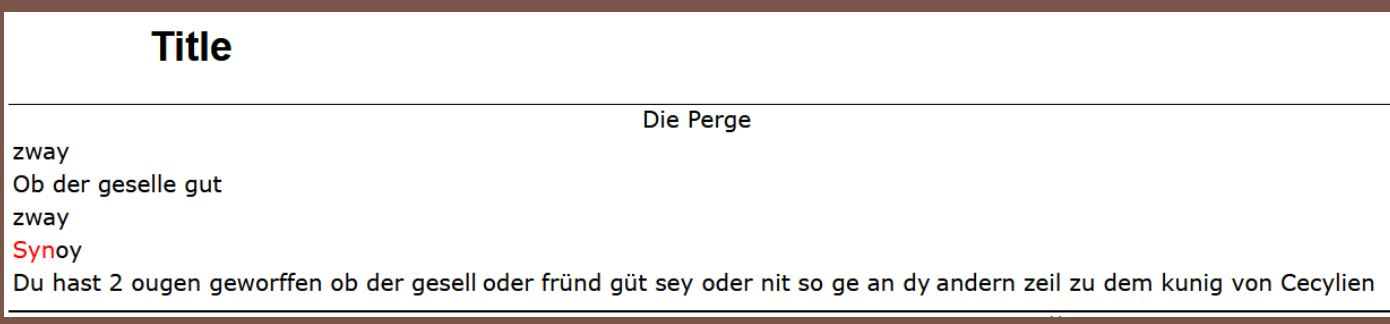
\includegraphics[width=0.9\textwidth]{abb-1-tei-parsed.JPG}
				\caption{HTML Darstellung der TEI-XML Struktur einer Scheibe.}
				\label{Abbildung 1}
			\end{figure}
			Das TEI Mark Up hierfür ist absichtlich einfach gehalten. Es setzt sich aus einer Tabelle zusammen, die die entsprechende
			Scheibe darstellt. Der TEI-XML Code sieht für dieses Beispiel folgendermaßen aus:
\vspace{5mm}			

\begin{lstlisting}[
    language=TEI-XML, 
    basicstyle=\ttfamily\small,    % Kleinere Schrift
    frame=single,         % Einfache Rahmenlinie
    caption={TEI-XML für den Ausschnitt einer Scheibe}, % Titel unter dem Listing
	captionpos=b,
    label={lst:tei-example}, % Label für Verweise im Text
    numbers=left,         % Zeilennummern links anzeigen
    numberstyle=\tiny,    % Sehr kleine Zeilennummern
    breaklines=true       % Zeilenumbruch bei langen Zeilen
]
<table rows="4" cols="4">
	<head>Die Perge</head>
	<row>
	   <cell>zway</cell>
	</row>
	<row>
	   <cell>Ob der geselle gut</cell>
	</row>
	<row>
	   <cell>zway</cell>
	</row>
	<row>
	   <cell><hi rend="red">Syn</hi>oy</cell>
	</row>
	<row>
	   <cell>Du hast 2 ougen geworffen ob der gesell</cell>
	   <cell>oder fründ güt sey oder nit so ge an dy</cell>
	   <cell>andern zeil zu dem kunig von Cecylien</cell>
	</row>
</table>
\end{lstlisting}
	
	\subsubsection{Interpretative Edition mit TEI-XML}
		Zuletzt wird eine Interpretative Edition angeboten. Hierdurch soll es Lesern ohne Fachkenntnisse der alten Sprachformen 
		ermöglicht werden, das Losbuch zu verstehen. TEI wird hierbei verwendet, um Ergänzungen erkenntlich zu machen, wie z. B. 
		ausgeschriebene Abkürzungen oder Einfügungen moderner Sprachformen. Diese Ergänzungen sollen dann in der Anwendung angezeigt 
		werden, wenn der Nutzer seinen Mauszeiger über das entsprechende Wort bewegt. Hierbei werden Abkürzungen automatisch erweitert oder 
		moderne Wortformen angezeigt in einem Kontextmenü angezeigt (Abb. 2). 
		Wenn für eine Abkürzung zudem eine moderne Wortform angegeben ist, wird diese in Klammern dahinter angezeigt (Abb. 3).
			\begin{figure}[htbp]
				\centering
				
\includegraphics[width=0.9\textwidth]{abb-2-tei-parsed-hover-ougen.JPG}
				\caption{Mouseover zeigt ein Kontextmenü}
				\label{Abbildung 2}
			\end{figure}
			\begin{figure}[htbp]
				\centering
				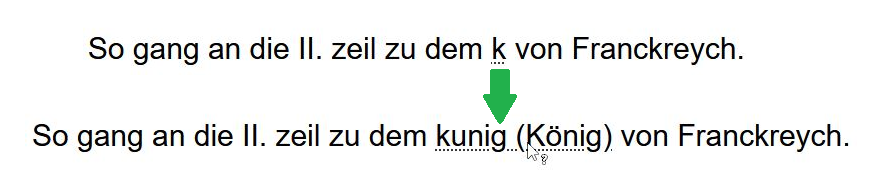
\includegraphics[width=0.9\textwidth]{k-kunig-koenig-onhover.png}
				\caption{Mouseover erweitert Abkürzung}
				\label{Abbildung 3}
			\end{figure}
	\subsection{Gestaltung des Benutzerinterfaces}
		\subsubsection{Navigations- und Einstellungsmöglichkeiten}
		Die im vorigen Kapitel erläuterten Elemente sollen über ein Benutzerinterface konfigurierbar sein. 
		Dieses Interface ist folgendermaßen aufgebaut: Auf jeder Seite gibt es Kontrollelemente wie Buttons und Toggles, 
		mit denen die visuellen Elemente ein- und ausgeblendet werden können. Abbildung 4 zeigt beispielhaft den Aufbau einer Seite mit 
		aktiviertem Faksimile und interpretativer Edition.\\
		Im Header befindet sich ein Toggle, um zwischen Editions- und Spielmodus zu wechseln (siehe nächstes Kapitel). 
		In der Mitte des Headers befindet sich ein Navigationsfeld für die Losbuchseiten samte eines Suchfeldes. Rechts 
		davon ein Dropdownmenü namens \textit{Ansicht}. In diesem Menü können die zuvor beschriebenen Editionsformen ausgewählt werden. 
		Wird dort nur der Modus \textit{Faksimile} angewählt, nimmt der Scan der Buchseite den gesamten Bereich der unteren Seite ein. 
		Wird zusätzlich noch eine der beiden anderen Editionsformen gewählt, kann dieser Modus neben dem Faksimile angezeigt werden. 
		So kann man jederzeit entscheiden, ob man zwei oder nur eine Ansicht aktiviert hat. Wenn nämlich der interpretative Modus ausgewählt wird,
		nachdem man zuvor schon den diplomatischen Modus aktiv hatte, erscheint kein zusätzliches Element auf der Seite, sondern die Ansicht des diplomatischen 
		Modus wird in den interpretativen Modus geschaltet. In einer Sidebar wird links die Möglichkeit geboten, die entsprechende Stelle zu vergrößern oder zu markieren.
			\begin{figure}[htbp]
				\centering
				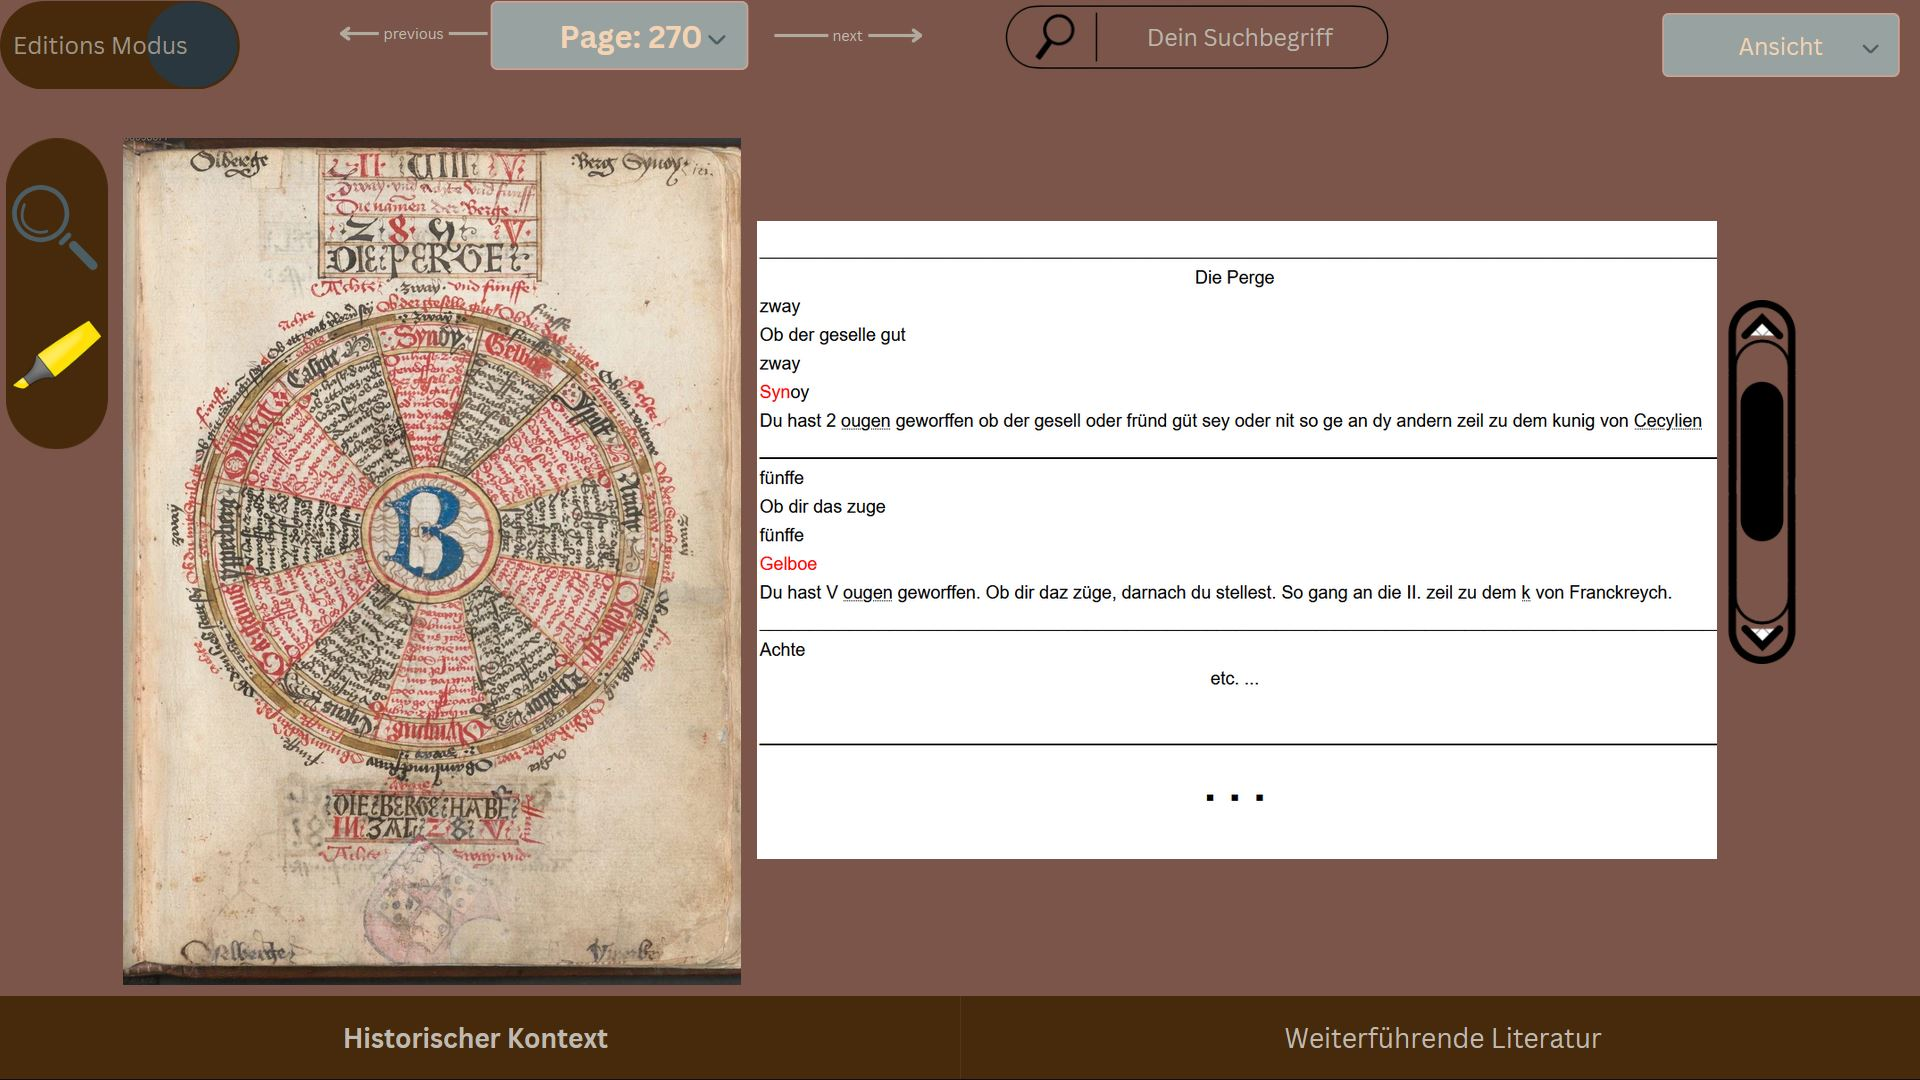
\includegraphics[scale=0.3]{ansicht-startseite-editionsmodus.JPG}
				\caption{Die Seite einer Scheibe im Editionsmodus}
				\label{Abbildung 4}
			\end{figure}

		\subsubsection{Interaktiver Spielmodus}
		Der Spielmodus bietet ein interaktives Erlebnis des Losbuches. Hier kann man direkt in der Webanwendung alle Schritte des Losbuchspiels aktiv ausführen.
		Es gibt zwei Varianten des Spiels: Einen \textit{Easy mode} und einen \textit{Hard mode}. Man beginnt auf der Seite mit den Fragen, von denen man eine per Klick 
		auswählt. Im \textit{Easy mode} werden die Fragen transkribiert in einer Liste angezeigt, wohingegen man im \textit{Hard mode} die Frage innerhalb des Faksimiles 
		anklicken muss. In beiden Spielvarianten ist ein Würfelbutton rechts plaziert um den Wurf zu generieren. Im \textit{Easy mode} erscheint nun ein neuer Button, den man 
		klickt, um direkt zur richtigen Scheibe zu gelangen. Im \textit{Hard mode} muss man nun selbst tätig werden und das Buch nach der Scheibe mit der richtigen Kombination
		von Zahl und Frage durchsuchen. Von dort aus setzt sich dieses Spiel dann so fort. Im \textit{Hard mode} muss man alles selbst suchen, im \textit{Easy mode} wird man über dokumentinterne Hyperlinks an die
		richtige Stelle weitergeleitet. Die Abbildungen 5 und 6 zeigen die Unterschiede jeweils auf. Im \textit{Hard mode} erhält man zudem die Möglichkeit, das Faksimile in den Vollbildmodus zu versetzen.
					\begin{figure}[htbp]
				\centering
				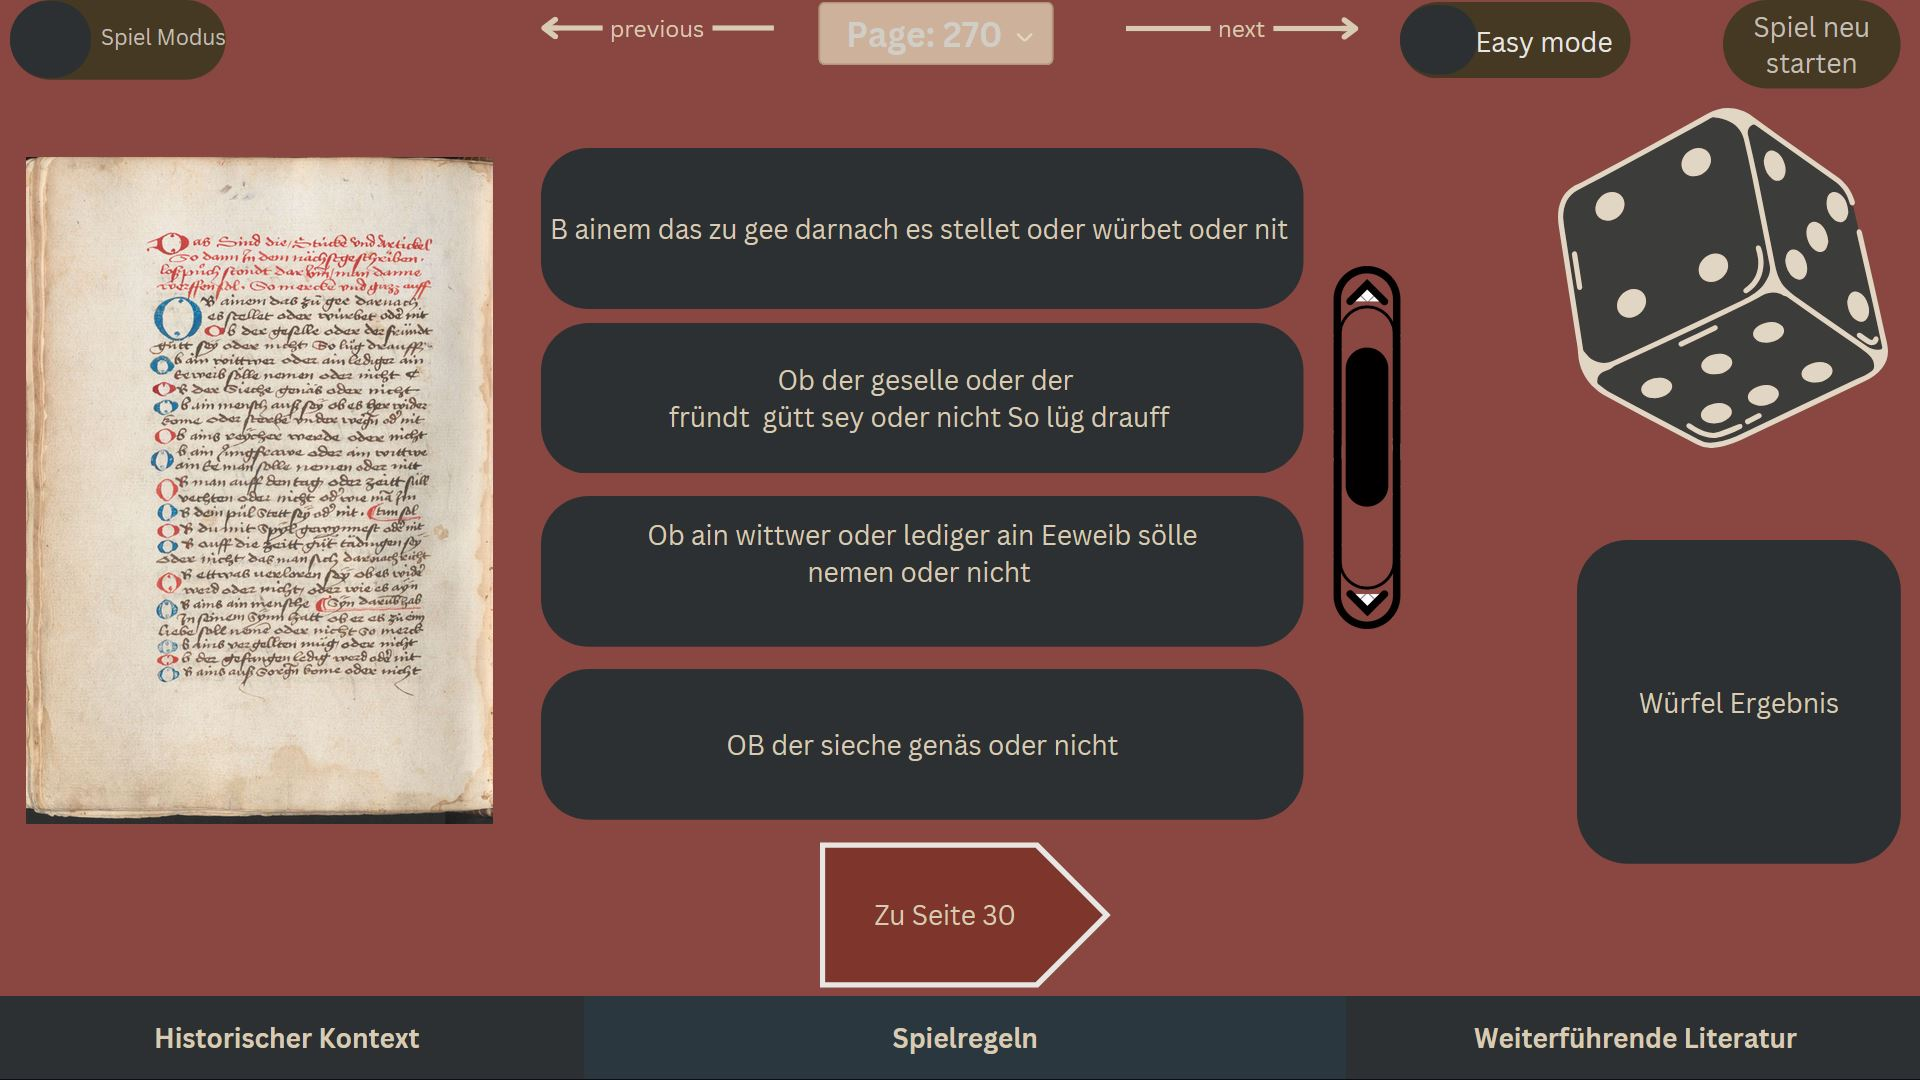
\includegraphics[scale=0.3]{ansicht-gamemodus-easy.JPG}
				\caption{Die Startseite im \textit{Easy mode} Spielmodus}
				\label{Abbildung 5}
			\end{figure}
			\begin{figure}[htbp]
				\centering
				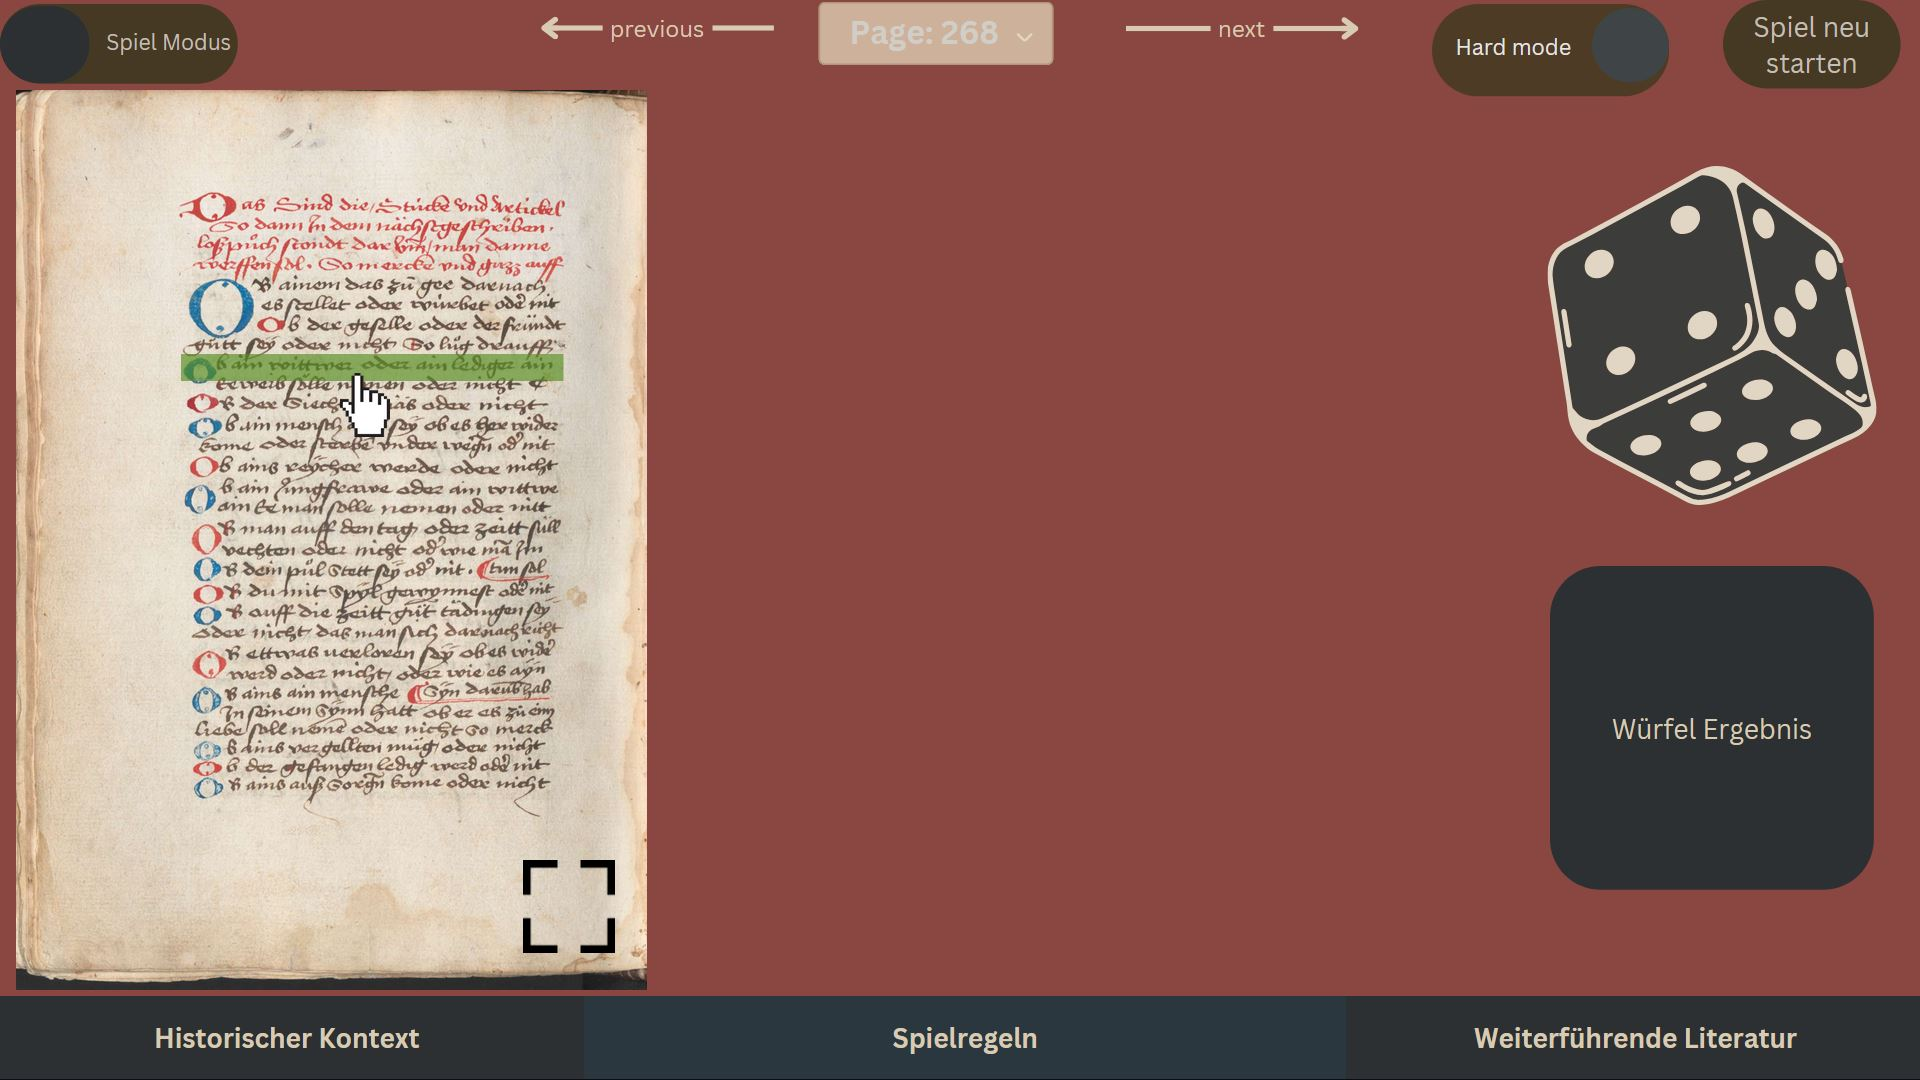
\includegraphics[scale=0.3]{ansicht-gamemodus-hard.JPG}
				\caption{Die Startseite im \textit{Hard mode} Spielmodus}
				\label{Abbildung 5}
			\end{figure}

\section{Zusammenfassung und Ausblick}


\printbibliography


\end{document}
